\chapter{Einleitung}\label{chap:einleit}
\section{Projektbeschreibung}\label{sec:projektbeschreibung}

In den Schulen ist die Mensa nicht immer gut. Man kann nie Wissen, ob das Essen
schmeckt, bis man es gekauft hat. Dieser Problemstellung widmet sich dieses
Projekt. Es soll das Essen an der Mensa der Neuen Kantonsschule Aarau bewerten
werden. Genauer soll das Essen von den Schülern/Kunden selbst bewertet werden.
Das soll mithilfe eines neuen Bewertungsportal in Form einer Webseite ermöglicht
werden. Dadurch kann man schon einen Blick auf das Essen erhaschen, bevor man es
gekauft hat.

Das Projekt ist insofern spannend, weil viele Schüler gar nicht mehr die Mensa
besuchen. Das liegt daran, dass sie bereits schlechte Erfahrungen mit dem Essen
gemacht haben. Vielleicht lässt sich mit diesem Projekt die Mensa verbessern und
die Schüler wieder in die Mensa locken.

Es gibt bereits schon viele verschiedene Bewertungsportale für Restaurants und
andere Geschäfte. Dennoch sollte dieses Projekt etwas speziell
zurechtgeschnittenes für die Mensa der Neuen Kantonsschule Aarau werden.
Aus diesem Grund ist diese Arbeit eine Engineering Arbeit.

Um diese Arbeit umzusetzen braucht es Kenntnise in den Bereichen:
\begin{itemize}
    \item Datenbanken
    \item Webseiten Frontend
    \item Webseiten Backend
    \item Design
    \item Netzwerke
    \item Webscraping
\end{itemize}

Die Arbeit nutzt für die Umsetzung folgende Technologien:
\begin{itemize}
    \item Libraries
    \subitem Django (Python Webserver Framework)
    \subitem Requests  (Zum senden von HTTP Anfragen)
    \subitem BeautifulSoup  (Zum analysieren von HTML Seiten)
    \subitem Datetime (Zum verarbeiten von Datum und Zeit)
    \subitem (Noch viele weitere, welche aber eine keine Hauptrolle in dem Projekt spielen)
    \item Sprachen
    \subitem Python (Backend)
    \subitem HTML (Design)
    \subitem CSS (Design)
    \subitem JavaScript (Frontend)
    \item IDE
    \subitem Visual Studio Code
\end{itemize}

\subsection{Architektur der Webseite}
\begin{figure}[ht]
    \centering
    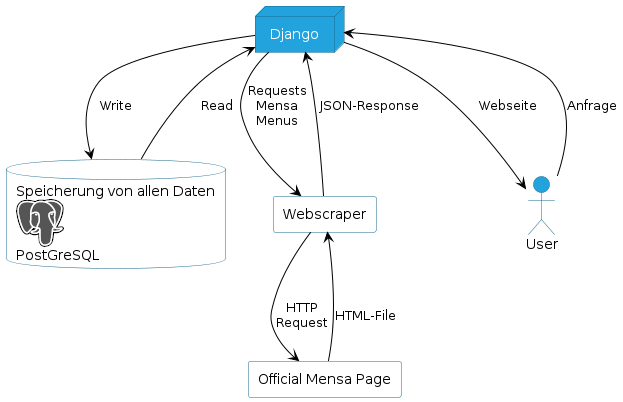
\includegraphics[width=0.8\textwidth]{images/Webseite.png}
    \caption{Architektur der Webseite}
    \label{fig:Website}
\end{figure}

Die Webseite besteht aus verschiedenen Teilen. Der Hauptteil ist der
\code{Django}-Server. Dieser macht die zentrale Arbeit. Die Anfragen der Nutzer
werden auch an diesen Server geschickt. \code{Django} arbeit dann mit der
Datenbank (\ref{sec:DB}) und dem Webscraper (siehe \ref{spez:Webscraper})
zusammen, um Daten zu beschaffen oder sie zu speichern.

\section{Problemdefinition}\label{sec:problemdefinition}

Die Grundanforderung für das Projekt sind:
\begin{itemize}
    \item Menus von der Mensa müssen geladen und angezeigt werden
    \item Bilder Gallerie, wo man die Bilder der Gerichte sehen, posten und liken kann
    \item Reviews vom Essen müssen gepostet, geliked und gesehen werden
    \item Das Essen muss mit einem Rating bewertet werden können
    \item Die Menus müssen nach verschiedene Kriterien sortiert/gefiltert werden können.
    \item Die Webseite braucht ein ansprechendes und einfaches Design
\end{itemize}

Damit das Projekt noch erfolgreicher wird, braucht es:
\begin{itemize}
    \item Account System
    \item Mobile Responsiveness für eine gute Nutzung auf Smartphones
    \item Ein Punktesystem (Karma) für qualitative Bewertungen
    \item Ein Achievement System, wobei User Bilder neben ihrem Namen verdienen können.
    \item Eine Veröffentlichung auf eine richtige Serverinfrastruktur
\end{itemize}
